\newpage
\section{\textit{Transformers} e LLM}

De acordo com a introdução de \textit{Transformers} dada pelo trabalho apresentado por \cite{vaswani2023attentionneed} o \textit{self-attention}, ou \textit{intra-attention}, é um mecanismo  que relaciona diferentes posições de uma única sequência para computar uma representação dessa sequência. A \textit{auto-attention} foi usada com sucesso em várias tarefas, como compreensão de leitura, sumarização abstrativa, implicação textual e aprendizado de representações de sentenças independentes da tarefa.

O Transformer introduz um conceito inovador ao reduzir as operações necessárias para relacionar duas posições de um vetor a um número constante. Isso é alcançado através do mecanismo de\textit{ self-attention}, que permite a computação constante independentemente da distância entre as posições na sequência do vetor. No entanto, esse processo pode levar a uma redução da resolução efetiva, já que a atenção média ponderada das posições dos vetores pode suavizar os detalhes finos das representações.

No \textit{Transformer}, a \textit{auto-attention} calcula a importância de cada posição na sequência em relação a todas as outras posições. Em outras palavras, ele pondera a contribuição de cada posição ao computar uma nova representação para cada posição. O problema surge porque essa ponderação é, essencialmente, uma média ponderada. Que especialmente ao considerar muitas posições, os detalhes específicos podem se perder. Similar ao tentar descrever uma paisagem detalhada olhando apenas para a média das cores em uma fotografia; é perdido perde as nuances e detalhes individuais.

Para mitigar essa redução na resolução efetiva, o \textit{Transformer} utiliza a \textit{Multi-Head Attention} \cite{vaswani2023attentionneed}. Esse mecanismo permite que o modelo foque em diferentes partes da sequência simultaneamente, proporcionando múltiplas "visões" da sequência e melhorando a capacidade do modelo de capturar dependências complexas e detalhadas entre posições distantes.

A grande inovação do Transformer reside no fato de ser o primeiro modelo de  a usar exclusivamente auto-atenção para computar representações de entrada e saída. Diferente dos modelos de RNNs ou convoluções alinhadas à sequência, o Transformer evita essas estruturas, o que contribui para uma maior eficiência computacional e capacidade de paralelização.

A estrutura utilizada pelo Transformer, contemplando os fatores \textit{Mult-Head Attention}, \textit{Self-attention} é representado pela Figura \ref{fig:transformer1}

\begin{figure}[H]
    \centering
    \caption{Arquitetura do Modelo Transformer}
    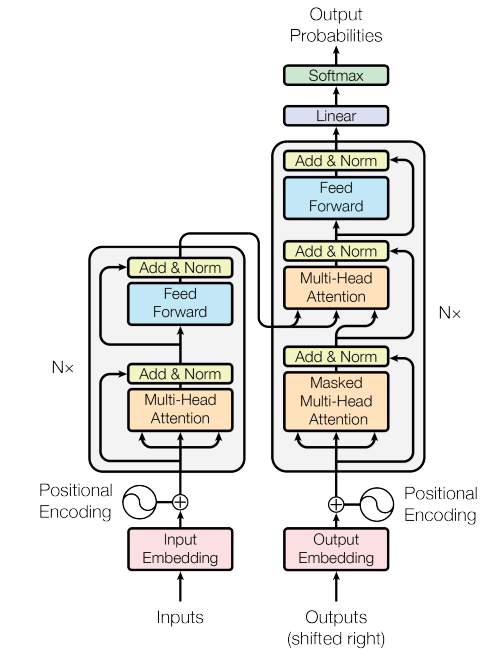
\includegraphics[width=\linewidth]{img/transformer1.png}
    \caption*{Fonte: \cite{vaswani2023attentionneed}}
    \label{fig:transformer1}
\end{figure}

\subsection*{\textit{Encoder}}
O codificador (encoder) do Transformer consiste em camadas $N = 6$. Cada camada tem dois subníveis: um mecanismo de \textit{self-attention} e \textit{multi-head attention} e uma rede \textit{feed-forward}.

No trabalho apresentado por \cite{vaswani2023attentionneed}, é realizado a normalização de camadas do transformer, seguido por uma saída de subnivel, representado pela Equação \ref{eq:layernorm}

\begin{equation}
\text{\textbf{LayerNorm}}(x + \text{\textbf{Sublayer}}(x))
\label{eq:layernorm}
\end{equation}

onde $\text{\textbf{Sublayer}}(x)$ é a função implementada pelo subnível. Para facilitar as conexões residuais, todos os subníveis e os \textit{embeddings} produzem saídas de dimensão $d_{\text{model}} = 512$.

\subsection*{\textit{Decoder}}

O decodificador (\textit{decoder}) também possui $N = 6$ camadas idênticas. Além dos dois subníveis do codificador, o decodificador adiciona um terceiro subnível para realizar atenção \textit{multi-head attention} sobre a saída do codificador. Assim como no codificador, utiliza-se conexões residuais e normalização de camada. O subnível de auto-atenção no decodificador é modificado para evitar que uma posição atenda a posições futuras. Essa máscara \ref{fig:transformer1}, juntamente com o deslocamento dos \textit{embeddings} de saída por uma posição, assegura que as previsões na posição $i$ dependam apenas das saídas conhecidas em posições menores que $i$.

\subsection*{Exemplo de Decodificação com Transformer}

Considerando um modelo Transformer treinado para tradução automática do inglês para o francês. Suponha que a frase de entrada em inglês seja:

\begin{quote}
\textit{The cat sat on the mat.}
\end{quote}

\subsection*{1. Entrada Codificada}

A frase de entrada é processada pelo codificador (\textit{encoder}) para gerar uma sequência de representações contínuas:

\[
\textbf{Z} = \{ \textbf{z}_1, \textbf{z}_2, \textbf{z}_3, \textbf{z}_4, \textbf{z}_5, \textbf{z}_6, \textbf{z}_7 \}
\]

onde cada \(\textbf{z}_i\) é uma representação contínua para cada palavra da frase "\textit{The cat sat on the mat.}"

\subsection*{Início da Decodificação}

O processo de decodificação começa com um token especial de início de sequência (por exemplo, \texttt{<start>}):

\[
\text{\textit{Input}}_\text{\textit{decoder}} = \{ \texttt{<inicio>} \}
\]

\subsection*{Geração da Primeira Palavra}

Usando a entrada \texttt{<inicio>}, o decodificador gera a primeira palavra da saída. Supondo que a palavra gerada seja "Le":

\[
\text{\textit{Output}}_\text{\textit{decoder}} = \{ \texttt{<inicio>}, \text{Le} \}
\]

\subsection*{Geração de Palavras Subsequentemente}

O \textit{token} "Le" é adicionado à entrada do decodificador e o processo é repetido. A sequência de entrada para o decodificador agora é:

\[
\text{\textit{Input}}_\text{\textit{decoder}} = \{ \texttt{<inicio>}, \text{Le} \}
\]

O decodificador gera a próxima palavra, por exemplo, "chat". Assim, a sequência de saída é atualizada para:

\[
\text{\textit{Output}}_\text{\textit{decoder}} = \{ \texttt{<inicio>}, \text{Le}, \text{chat} \}
\]

\subsection*{Repetição do Processo}

O \textit{decoder} continua esse processo até encontrar um token de fim de sequência (por exemplo, \texttt{<fim>}):

\[
\text{\textit{Final Output}}_\text{\textit{decoder}} = \{ \texttt{<inicio>}, \text{Le}, \text{chat}, \text{est}, \text{assis}, \text{sur}, \text{le}, \text{tapis}, \texttt{<fim>} \}
\]

Neste exemplo, o decodificador traduz a frase em inglês "\textit{The cat sat on the mat}" para o francês "\textit{Le chat est assis sur le tapis}". O processo envolve iniciar com um token especial, gerar palavras sequencialmente e usar a atenção para considerar as representações codificadas da frase original. Cada palavra gerada é adicionada ao contexto, e a sequência é ajustada até que o token de fim de sequência seja produzido.


\subsection*{Equação de \textit{Attention}}
Primeiro, calculamos o produto das matrizes de consultas \textbf{Q} e chaves \textbf{K} transposta, dado por \( QK^T \). Com o resultado de \( QK^T \), é normalizado dividindo cada elemento pelo valor \(\sqrt{d_k}\). Após isso, é realizada a aplicação da função \(\text{softmax}\left(\frac{QK^T}{\sqrt{d_k}}\right)\), para converter esses valores em probabilidades, ou "pesos" que somam 1.
Finalmente, esses pesos são multiplicados pela matriz de valores \textbf{V} para obter a saída final
\(\text{Attention}\textbf{(Q, K, V}) = \text{softmax}\left(\frac{QK^T}{\sqrt{d_k}}\right) V\).
A Equação \ref{eq:attention} representa a formula completa da Função \textit{Attention} por:
\begin{equation}
\text{\textit{Attention}}(\textbf{Q, K, V}) = \text{softmax}\left(\frac{\textbf{QK}^T}{\sqrt{d_k}}\right) \textbf{V}
\label{eq:attention}
\end{equation}


%================================================================================
% BERT================================================================================



\subsection{BERT - Transformação e predição de linguagem }
\label{bert}
Um dos marcos do desenvolvimento de LLM, é a utilização de \textit{Transformers}, com isso o Google \cite{DBLP:journals/corr/abs-1810-04805} deu a introdução ao modelo BERT \textit{(Bidirectional Encoder Representations from Transformers)}. Essa apresentação possibilitou uma sequencia de ganhos e desenvolvimentos posteriores no mundo de Machine Learning, impulsionou o desenvolvimento de sistemas de Perguntas e Respostas, Classificação de Texto, sistemas de busca, e também como ajudar na classificação de entidades-objeto de contextos de  software. A Figura \ref{fig:bert1} é representada pelo fluxo do LLM, com fins de interpretação e geração de texto, dado um \textit{text input} (ou \textit{prompt}), o modelo BERT realiza a tradução e transformação do conteudo, gerando uma representação numérica e o texto de saída \textit{Text Output}.

\begin{figure}[H]
    \centering
    \caption{Fluxo de LLM para transformação de texto.}
    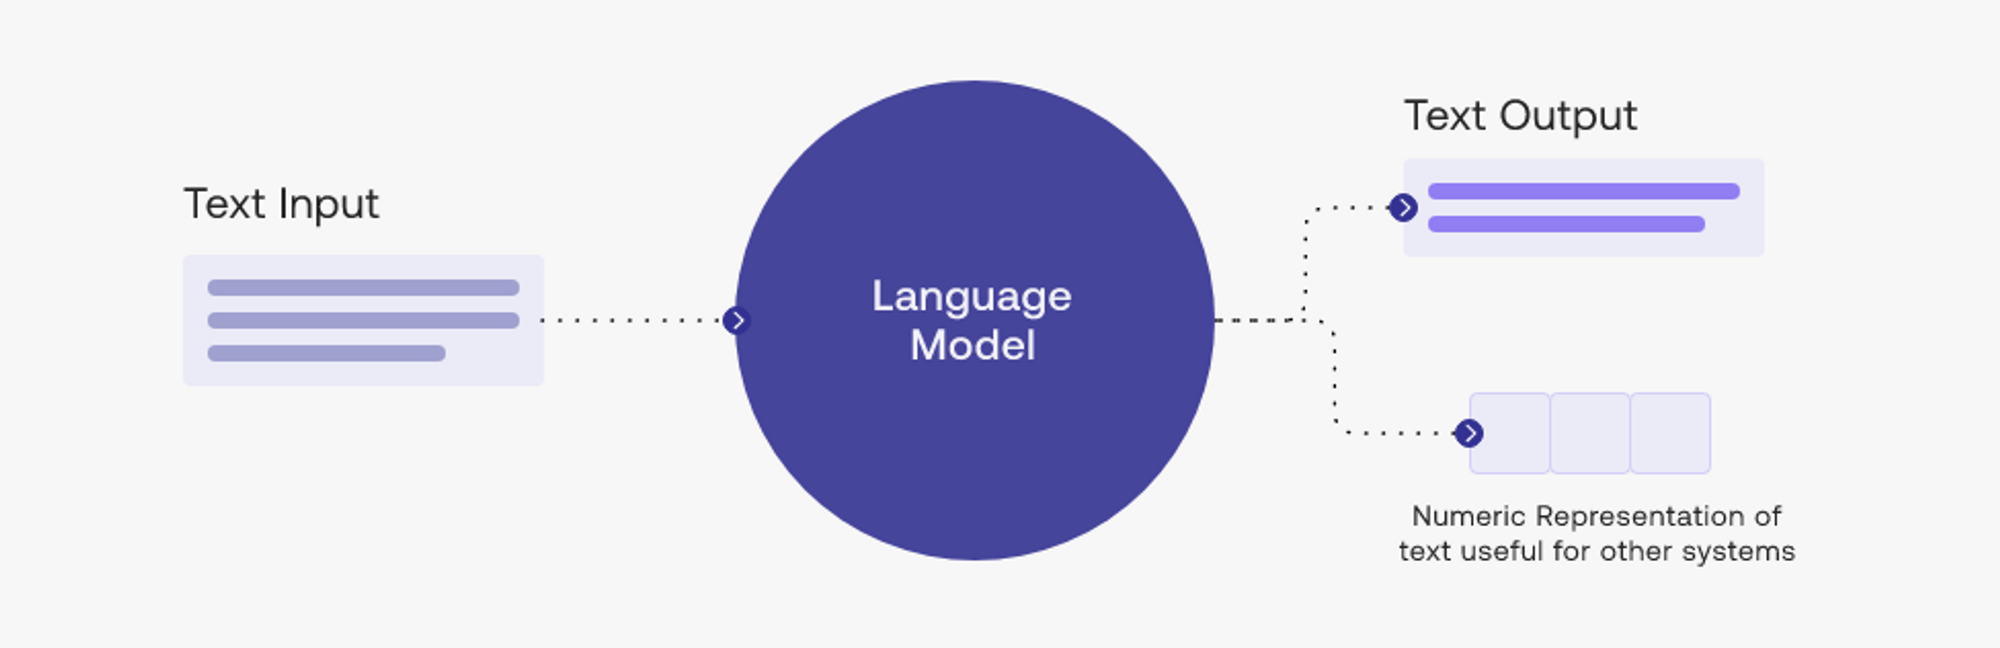
\includegraphics[width=\linewidth]{img/BERT/bert1.png}
    \caption*{ Fonte: attri.ai \cite{Attri2024}}
    \label{fig:bert1}
\end{figure}

\subsection{Visão geral do BERT}

BERT é um LLM  que é treinado baseado rede neural e concebido no contexto de \textit{transformers}, capaz de realizar transformações no texto para o contexto de linguagem. O modelo é Pré treinado baseado em aprendizagem não supervisionada, e após o treinamento, é feito o\textit{ fine tuning} no qual os dados são supervisonados com base em 
 uma saída alvo ou rótulo. Existem duas principais estratégias de treinamento \textit{self-supervised} do modelo:
 
\subsubsection{\textit{Masked Language Modeling} (MLM)}
Essa abordagem, faz o treinamento do modelo a partir da  da frase de entrada, uma porcentagem \% dos \textit{tokens}, definida para cada estratégia de treinamento,  são cobertos por um \textit{token} especial dado por [MASK] e o objetivo do modelo, é prever a parte que foi ocultada da frase, dado o contexto das palavras. Os pré requisitos para o \textit{fine tuning} desse comportamento, é dado pela sequencia a seguir: 

\begin{itemize}
    \item Na saída do modelo é necessária uma camada de classificação;
    \item Os vetores de saída são multiplicados pela matriz de \textit{embedding};
    \item Realiza o cálculo de cada palavra do texto, utilizando a função Softmax.
\end{itemize}

Na Figura \ref{fig:bert2} é mostrada a entrada dos \textit{tokens} dados por \textit{w1,w2,w3...}, [MASK] sendo a palavra mascarada, e por fim os \textit{embeddings} gerados após a camada de classificação, dados por \textit{w1', w2', w3'}.
\begin{figure}[H]
    \centering
    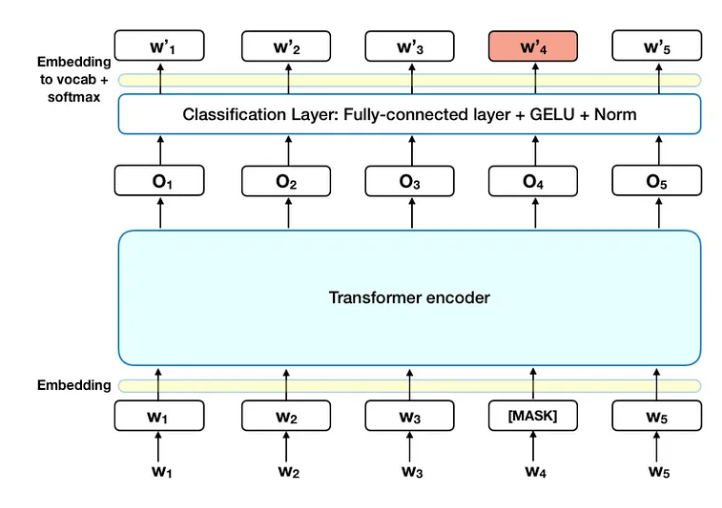
\includegraphics[width=\linewidth]{img/BERT/bert2.png}
    \caption{Arquitetura e Camadas do BERT para MLM, sendo elas: parâmetros de entrada, camada de transformação, camada de classificação}
    \label{fig:bert2}
\end{figure}

A função Softmax, dada pela Equação \ref{instance:eq:2}, converte um vetor de valores em probabilidades. Nesta equação, \({P_i}\) é a probabilidade da classe \(i\). O numerador \(e^{S \cdot T_i}\) é a exponencial do valor \(T_i\) da classe \(i\), ajustado por um fator de escala \(S\). O denominador \(\sum_{j} e^{S \cdot T_j}\) é a soma das exponenciais de todos os valores \(T_j\), garantindo que as probabilidades somem 1. O fator \(S\) controla a suavidade da distribuição.

\begin{equation}
    \label{instance:eq:2}
    {Pi} = \frac{e^{S \cdot T_i}}{\sum_{j} e^{S \cdot T_j}}
\end{equation}

A probabilidade da palavra \textit{Pi} estar classificada no intervalo de resposta dada o \textit{prompt} de texto de entrada, é calculado como um produto escalar entre Ti e S. O intervalo da probabilidade é calculado entre as posições \textit{\textbf{i}} e \textit{\textbf{j}} do vetor, que define o resultado da previsão.

Na Tabela \ref{tab:tab1} são exemplificados os formatos de textos de \textit{input} e \textit{output} para a operação de MaskedLM.


\begin{table}[H]
    \centering
    \caption{Exemplos de entrada e saída para o contexto de\textit{ Masked Language}, sendo \textit{P} a Probabilidade e [MASK] a palavra ocultada pelo modelo para que seja prevista.}
    \begin{tabularx}{\textwidth}{XXXXX}
    \hline
        \textbf{Texto de entrada} & \textbf{Texto de saída} & \textbf{\textit{P (word-1)}} & \textbf{\textit{P (word-2)}} &\textbf{\textit{P (word-3)}} \\ \hline
     \textit{United States is the \textbf{[MASK]} country of the world}  & \textit{United States is the \textbf{southernmost} country of the world} & \textit{southernmost}: 0.147 & \textit{northernmost}: 0.121 & \textit{largest}: 0.097 \\ 
     N\textit{eymar is the \textbf{[MASK]} of soccer} &\textit{ Neymar is the \textbf{father} of soccer} & \textit{father}: 0.284 & \textit{director}: 0.178 & \textit{president}: 0.057 \\ 
    \textit{Brazil the\textbf{ [MASK]} football team in the world} & \textit{Brazil the \textbf{best} football team in the world}  & \textit{best}: 0.505 & \textit{oldest}: 0.122 & \textit{youngest}: 0.068 \\ 
    \textit{ The \textbf{[MASK]} of the world} &\textit{ The \textbf{end} of the world}  & \textit{end}: 0.268 & \textit{future}: 0.023 & \textit{beginning}: 0.016 \\ \hline
    \end{tabularx}
    \caption*{Fonte: Do Autor}
    \label{tab:tab1}
\end{table}


\subsubsection{\textit{Next Sentence Prediction (NSP)}}

Na fase de pré treinamento do BERT, ele é adaptado a realizar uma previsão de uma próxima sentença ou frase realizando uma classificação binária. Dada duas sentenças A e B, e as respectivas classes (\textit{labels}) de classificação são dadas pelo criador do modelo \cite{DBLP:journals/corr/abs-1810-04805} como \textbf{\textit{IsNext}} e \textbf{\textit{NotNext}}.
Para as classificações como a sentença B sendo \textbf{\textit{NotNext}}, é atribuído o valor de uma sentença aleatória dentro do documento, assim como para as classificações de \textbf{\textit{IsNext}} são dadas à frases B são seguidas e complementares de A em 50\% dos casos. A Figura \ref{fig:bert3} representa o método de classificação do BERT e as respectivas sentenças.

\begin{figure}[H]
    \centering
    \caption{Estrurura de representação semantica das camadas de geração de \textit{embeddings} do BERT, dado duas senteças A e B.}
    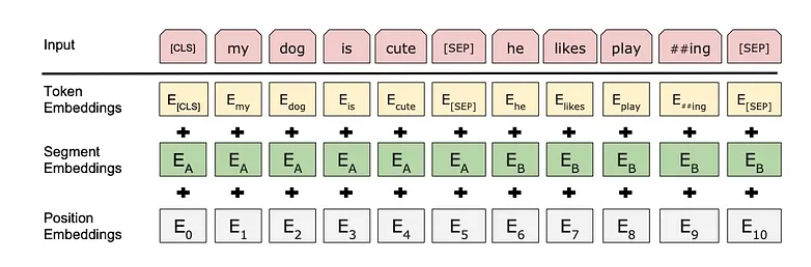
\includegraphics[width=\linewidth]{img/BERT/bert3.png}
    \caption*{Fonte: \cite{DBLP:journals/corr/abs-1810-04805}}
    \label{fig:bert3}
\end{figure}


A fase de pré-treinamento do BERT envolve duas tarefas principais: \textit{Masked Language Modeling} (MLM) e \textit{Next Sentence Prediction} (NSP), que se combinam para fortalecer a capacidade do modelo em entender o contexto das palavras e a relação entre sentenças. O MLM funciona mascarando uma porcentagem dos tokens de entrada com o token especial [MASK], e o objetivo do modelo é prever esses tokens mascarados com base no contexto fornecido pelas outras palavras na frase. 

Por outro lado, a NSP é uma tarefa de classificação binária onde o modelo recebe duas sentenças, A e B  \ref{fig:bert3}. Essa tarefa treina o modelo para captar a relação semântica entre sentenças consecutivas. A combinação dessas duas tarefas permite ao BERT ser aprimorado em representações contextuais das palavras, além de capturar informações de coerência entre sentenças. Isso traz uma maior robustez de geração de linguagem para o modelo, que pode ser adaptado (\textit{fine-tuned}) para uma variedade de tarefas de compreensão de linguagem natural, como \textit{question answering} e análise de sentimento.

\subsection{BERT \textit{base} e BERT \textit{large}}
Atualmente, existem muitas versões do BERT pré-treinado disponíveis, cada uma adaptada para diferentes aplicações e necessidades. No entanto, no artigo original publicado pelo Google, foram apresentadas duas versões principais do BERT: BERTbase e BERTlarge. Essas versões diferem significativamente em suas arquiteturas neurais e capacidade de processamento.

O BERTbase foi desenvolvido com uma arquitetura composta por 12 camadas de transformadores (também conhecidas como camadas de codificadores), cada uma com 12 camadas de atenção. No total, esta configuração resulta em 110 milhões de parâmetros treináveis. Essa versão foi projetada para ser mais leve e eficiente, facilitando seu uso em uma variedade de tarefas sem demandar excessivamente recursos computacionais.

Por outro lado, o BERTlarge apresenta uma arquitetura muito mais robusta. Ele possui 24 camadas de transformadores e 16 camadas de atenção em cada camada. Essa configuração expansiva leva o BERTlarge a um total impressionante de 340 milhões de parâmetros. Como esperado, o aumento significativo na complexidade e no número de parâmetros permite ao BERTlarge capturar nuances mais finas e realizar inferências mais precisas, resultando em um desempenho superior em diversos \textit{benchmarks} de compreensão de linguagem natural.

Nos testes de precisão, o BERTlarge demonstrou um avanço notável em relação ao BERTbase \cite{joshi2019bertcoreferenceresolutionbaselines}, evidenciando que a profundidade e a capacidade do modelo são fatores críticos para o sucesso em tarefas complexas de processamento de linguagem natural. Essa diferença de desempenho é particularmente notável em tarefas que requerem um entendimento profundo do contexto e da semântica, como resposta a perguntas, análise de sentimentos e tradução automática.

A criação dessas duas versões do BERT foi um marco significativo no campo da inteligência artificial e do processamento de linguagem natural, abrindo caminho para uma nova era de modelos de linguagem pré-treinados. A pesquisa e os desenvolvimentos subsequentes baseados no BERT continuaram a expandir e refinar essas ideias, resultando em uma proliferação de modelos derivados, cada um otimizado para diferentes aplicações e contextos específicos. A Figura \ref{fig:bert4} representa o gráfico comparativo entre  BERTlarge e BERTbase, dado para cada um deles, a quantidade de \textit{encoders}, a quantidade de \textit{self-attention heads}, dimensionalidade dos \textit{embeddings}, e total de parâmetros.

\begin{figure}[H]
    \centering
    \caption{Comparativo do BERTbase e BERTlarge.}
    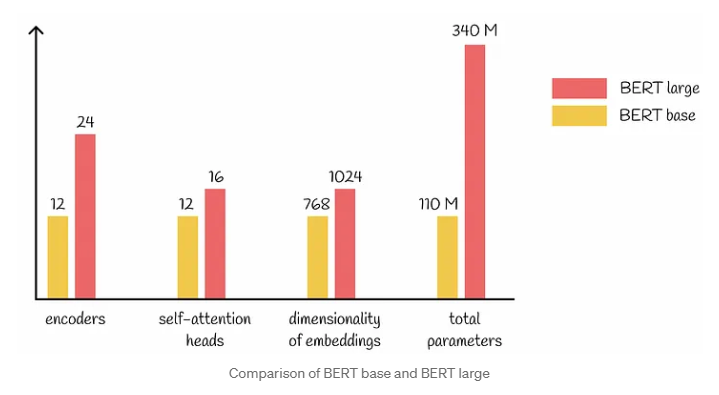
\includegraphics[width=\linewidth]{img/BERT/bert4.png}
    \caption*{Comparativo do BERTbase e BERTlarge. Fonte: Medium \cite{Rani2018}}
    \label{fig:bert4}
\end{figure}

\subsection{\textit{Fine Tunning}}
Em toda sua etapa de construção, o BERT passa por duas etapas, sendo elas Pré treinamento e \textit{fine tuning}. Todavia, após a modelagem ter sido consolidada, o BERT pode ser utilizado para realizar tarefas específicas, e com isso, novos métodos de \textit{fine tuning} podem ser realizados de acordo com o objetivo da tarefa.

Alguns casos de aplicação sugerem a aplicação do BERT para Classificação de Texto, Perguntas e Respostas, e também como auxílio em fluxos de RAG (\textit{Retrieval Augmented Generation}). Devido à sua camada probabilistica, como mencionado no tópico 2.1.2 deste texto, a partir de uma camada de \textit{fine tuning}, o BERT pode ser utilizado para geração de \textit{Embeddings} vetoriais, com o fim de trazer o benefício esperado para a tarefa em específica.

\subsection{BERT no contexto \textit{Question and Answering}}
Por sua vez, o BERT pode ser utilizado como um modelo fundamental para a geração de texto. Através de etapas de \textit{fine tuning}, o BERT se torna um poderoso gerador de texto em um determinado contexto, visto que a etapa de \textit{Generation} se da a partir a tarefa de \textit{Next Sentence Prediction}.

Para encontrar respostas no parágrafo, o BERT recebe uma pergunta e um parágrafo, gerando \textit{embeddings} para todos os \textit{tokens}. O modelo calcula o produto escalar entre cada \textit{embedding} do parágrafo e um vetor treinável \( T_{\text{start}} \), normalizando esses valores com a função \textit{softmax} \ref{softmax} para obter probabilidades. O \textit{token} com a maior probabilidade é considerado o início da resposta.

O processo para prever o \textit{token} final da resposta é semelhante. Utiliza-se um vetor treinável \( T_{\text{end}} \) para calcular produtos escalares com os \textit{embeddings} do parágrafo, normalizados com softmax \ref{softmax}. O token com a maior probabilidade é considerado o fim da resposta.

Para treinar o modelo, utiliza-se a distribuição de probabilidade verdadeira para calcular a perda (\textit{loss}) e ajustar os pesos do modelo através da backpropagação. Isso melhora a precisão da previsão das posições de início e fim da resposta, permitindo ao BERT extrair respostas precisas de um parágrafo com base na pergunta dada. Essa estrutura é representada pela Figura \ref{fig:bert5}

\begin{figure}[H]
    \centering
    \caption{BERT no contexto Q\&A (\textit{Question and Answering)}.}
    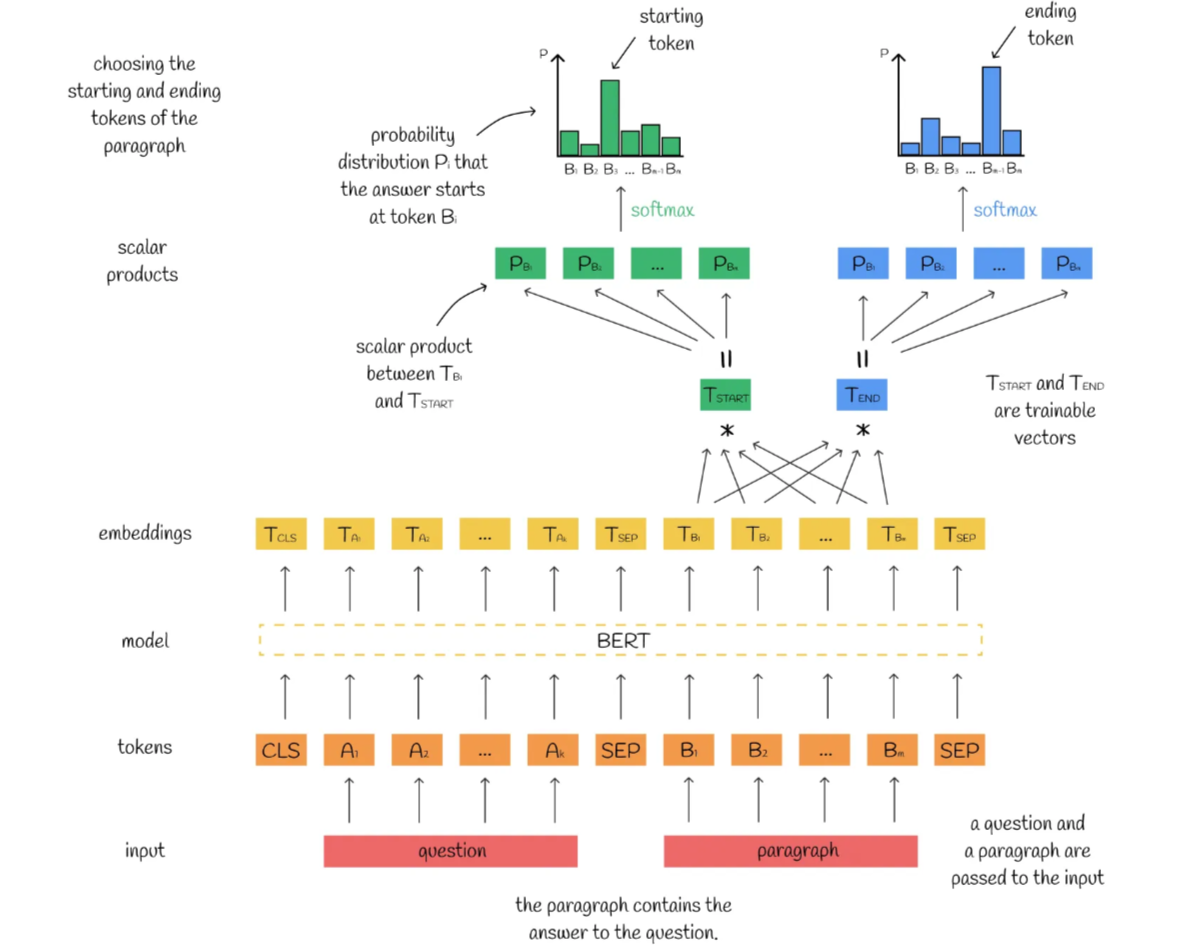
\includegraphics[width=\linewidth]{img/BERT/bert5.png}
    \caption*{Fonte: Towards Data Science \cite{Rani2018}}
    \label{fig:bert5}
\end{figure}

A partir de um \textit{Input} (\textit{question}) ou \textit{prompt} o BERT associa as palavras de entrada como sendo \textit{Tokens}, que acabam se tornando palavras vetorizadas e tratadas. Por sua vez, o papel do [SEP] é a divisão entre a questão de entrada e o conjunto de texto no qual a informação esteja relacionada.

Após a geração de \textit{tokens}, a entrada no modelo são os \textit{token} de \textit{query} contendo a informação de pergunta e \textit{paragraph} com o conteudo, na saída são calculados os \textit{embeddings} diante de cada \textit{token} da \textit{query} para cada documento presente no conteúdo de entrada. Esse calculo é feito a partir de um produto escalar (multiplicação entre dois vetores que tem como resultado uma grandeza escalar) entre cada \textit{token} de ambas as sentenças, gerando um valor numérico representado por uma probabilidade. A Equação \ref{eq:dot_product} representa o cálculo da multiplicação entre dois vetores, \cite{Bechtel1971} \( \mathbf{a} \cdot \mathbf{b} \).

\begin{equation}
    \label{eq:dot_product}
    \mathbf{a} \cdot \mathbf{b} = \sum_{i=1}^{n} a_i b_i
\end{equation}

\subsection{Utilização do SENTENCE-Bert (SBERT) para geração de \textit{Embeddings}}

O BERT tornou-se uma ferramenta amplamente utilizada em uma variedade de tarefas de processamento de linguagem natural, como análise de sentimentos e resposta a perguntas. Além dessas aplicações, o BERT é cada vez mais valorizado para a criação de \textit{embeddings} de palavras - vetores numéricos que capturam os significados semânticos das palavras.

Por exemplo, na análise de sentimentos, o BERT pode ser utilizado para determinar o tom emocional de um texto, como classificar uma avaliação de produto como positiva ou negativa. Em sistemas de resposta a perguntas, o BERT pode interpretar uma pergunta e encontrar a resposta mais relevante em um \textit{corpus} de documentos.

Além disso, os \textit{embeddings} gerados pelo BERT são usados em tarefas de similaridade semântica, onde a proximidade entre os vetores representa a similaridade no significado das palavras. Isso é útil em aplicações como a pesquisa de informações, onde o objetivo é encontrar documentos ou passagens que sejam semanticamente semelhantes à consulta do usuário, ou em sistemas de recomendação, onde os itens recomendados são aqueles que têm maior afinidade semântica com as preferências do usuário.

Dessa forma, o BERT não só aprimora a precisão em várias tarefas de NLP (\textit{Natural Language Processing}), mas também facilita a construção de representações semânticas ricas que podem ser aplicadas em diversos contextos.

De acordo com o estado da arte do SBERT (Sentence-BERT) \cite{reimers2019sentencebertsentenceembeddingsusing}, este modelo pode ser utilizado em uma ampla gama de tarefas, incluindo classificações, regressões, análise de sentimentos, entre outras. O SBERT é capaz de realizar \textit{fine tuning} tanto de maneira supervisionada quanto não supervisionada, o que aumenta sua versatilidade e eficácia em diferentes aplicações.

Em tarefas de classificação, o SBERT pode categorizar textos em diversas classes, como identificar tópicos de discussão ou determinar a polaridade de opiniões. Em regressão, ele pode ser usado para prever valores contínuos, como a previsão de notas em resenhas de produtos. Na análise de sentimentos, o SBERT é eficaz em detectar e avaliar as emoções expressas em textos.

Além disso, o \textit{fine tuning} supervisionado permite que o SBERT seja adaptado para tarefas específicas ao treinar o modelo com dados rotulados. Já o \textit{fine tuning} não supervisionado pode ser realizado através de métodos como o aprendizado contrastivo, onde o modelo aprende a partir das relações entre os pares de textos sem a necessidade de rótulos explícitos.

Essas capacidades tornam o SBERT uma ferramenta poderosa e flexível para várias aplicações de processamento de linguagem natural.

Para tarefas do escopo de RAG, a geração de \textit{embeddings} pode ser baseada na arquitetura do SBERT como sendo contextualizado para uma tarefa de classificação, tendo em vista que nesse contexto o modelo trabalhará em uma situação probabilística a partir da proximidade de vetores.

\subsubsection{SBERT para tarefas de classificação}
\label{softmax}
\begin{figure}[H]
    \centering
    \caption{Arquitetura do SBERT aplicado à tarefas de classificação.}
    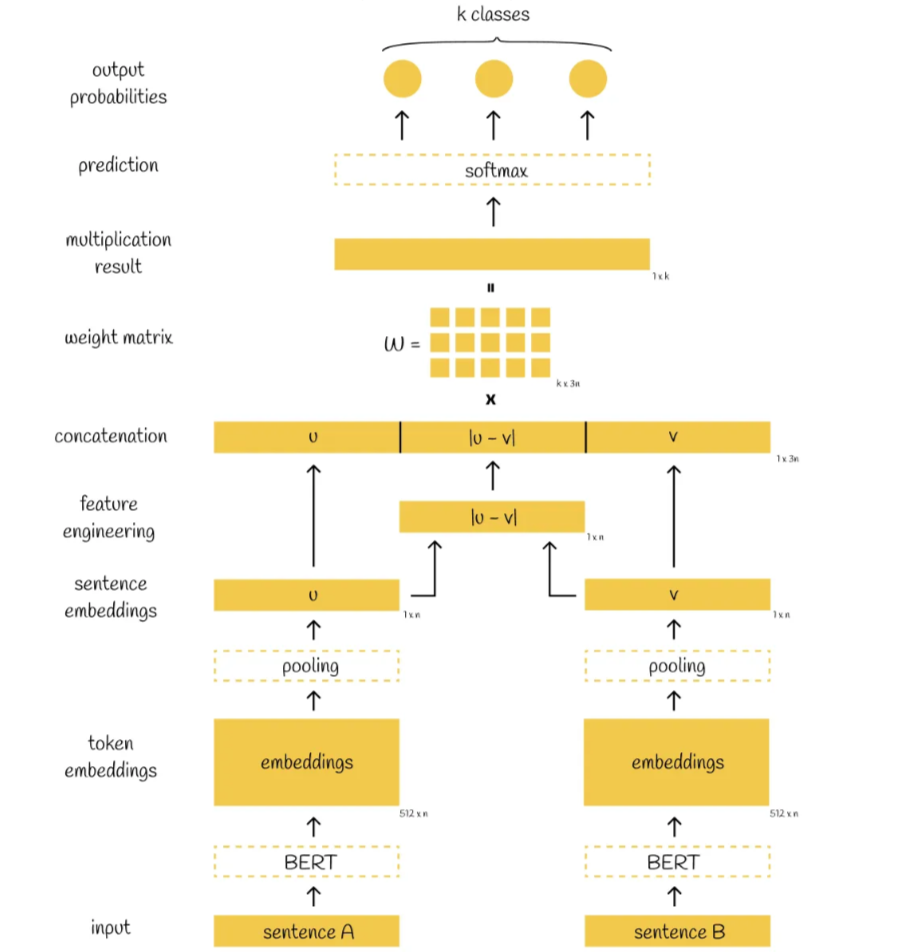
\includegraphics[width=\linewidth]{img/BERT/bert7.png}
    \caption*{Fonte: Towards Data Science \cite{Vyacheslav2023}}
    \label{fig:bert7}
\end{figure}

Os parâmetros de entrada são \textbf{Sentence A} e \textbf{Sentence B}, dos quais passam pela primeira etapa arquitetural do BERT e cada sentença tem seu resultado organizado por \textit{Embeddings} de \textit{Tokens}.
Após essa etapa de transformação, os parâmetros de configuração para classificação do SBERT são por \(\boldsymbol{\upsilon}\) e \(\boldsymbol{\nu}\).
Após a etapa de criação de \textit{embeddings}, os vetores \(\boldsymbol{\upsilon}\) e  \(\boldsymbol{\nu}\) são concatenados em um elemento absoluto com a diferença de  \(\boldsymbol{\upsilon}\) - \(\boldsymbol{\nu}\). Essa concatenação combina efetivamente as informações de ambos os \textit{embeddings} de frases, bem como suas diferenças, capturando o quão semelhantes ou diferentes as frases são.

O vetor concatenado é multiplicado por uma matriz de pesos \( W_t \) com dimensões \( 3n \times k \), onde \( n \) é o número de características do vetor e \( k \) é o número de possíveis \textit{labels} ou classes em uma tarefa de classificação. Na fórmula, \( W_t \) é a matriz de pesos que transforma o vetor concatenado em uma representação de classe. Especificamente, \( W_t \) tem dimensões \( 3n \times k \), indicando que ela projeta o vetor concatenado, que possui \( 3n \) elementos, para um espaço com \( k \) dimensões, correspondentes às classes ou labels possíveis.


A formula da matriz de peso é dada pela Equação \ref{eq:weigth_matrix} \cite{reimers2019sentencebertsentenceembeddingsusing}: 

\begin{equation}
    \label{eq:weigth_matrix}
   W_t \in \mathbb{R}^{3n \times k}
\end{equation}

O resultado da equação da multiplicação da matriz, é dado pelo vetor  \(\boldsymbol{\theta}\) que passará por uma Equação \ref{eq:softmax} de ativação Softmax, dada por \cite{reimers2019sentencebertsentenceembeddingsusing}:

\begin{equation}
    \label{eq:softmax}
    \boldsymbol{\theta} = \text{softmax}(W_t [\boldsymbol{\upsilon}, \boldsymbol{\nu}, |\boldsymbol{\upsilon} - \boldsymbol{\nu}|])
\end{equation}

A função softmax converte o vetor k-dimensional em uma distribuição de probabilidade sobre o \textit{k} classes possíveis. A saída da função softmax fornece as probabilidades previstas para cada classe.
O modelo é treinado otimizando a perda de entropia cruzada. A perda de entropia cruzada mede a diferença entre a distribuição de probabilidade prevista (obtida da função softmax) e a distribuição verdadeira (os rótulos reais)
\cite{reimers2019sentencebertsentenceembeddingsusing}.
Ao minimizar a perda de entropia cruzada, o modelo aprende a fazer previsões precisas para a tarefa de classificação.


\subsubsection{Arquitetura de inferência}

Para a arquitetura de inferência, o fluxo até a geração dos vetores $\upsilon$ e $\nu$ são similares, entretanto, ao invés de serem unificados para posteriormente multiplicados, logo são atribuídos a uma função de similaridade do coseno, para gerar as similaridades entre os vetores e obter os scores dos \textit{embeddings}.

Os vetores \(\boldsymbol{\upsilon}\) e \(\boldsymbol{\nu}\) passam pela Função de Similaridade do Coseno, sendo representada pela Equação \ref{eq:cosinesim}: 

\begin{equation}
    \text{cosine similarity} = \frac{\boldsymbol{\upsilon} \cdot \boldsymbol{\nu}}{\|\boldsymbol{\upsilon}\| \|\boldsymbol{\nu}\|} = \frac{\sum_{i=1}^{n} \boldsymbol{\upsilon}_i \boldsymbol{\nu}_i}{\sqrt{\sum_{i=1}^{n} \boldsymbol{\upsilon}_i^2} \sqrt{\sum_{i=1}^{n} \boldsymbol{\nu}_i^2}}
    \label{eq:cosinesim}
\end{equation}

\subsection{Vantagens e Limitações}

De acordo com o contexto apresentado no presente texto sobre o BERT e SBERT, as vantagens observadas da modelagem e \textit{fine tuning}, seguem representativamente por:

\begin{itemize} 
    \item \textbf{Mapeamento vetorial aprimorado:} SBERT melhora a forma como as sentenças são representadas no espaço vetorial, melhorando a compreensão semântica;
    \item \textbf{Desempenho:} Gera os \textit{embeddings} em várias tarefas de similaridade semântica aprimorada;
    \item \textbf{Versatilidade:} Lida com tarefas computacionalmente intensas, como \textit{clustering}, com tempo de computação significativamente reduzido;
\end{itemize}


\begin{itemize} 
 \item \textbf{Dependência do BERT:} Depende fortemente do BERT como modelo base, limitando a flexibilidade e adaptabilidade;
 \item \textbf{Eficácia específica da tarefa:} Os benefícios podem não ser traduzidos uniformemente em todas as aplicações de NLP;
 \item \textbf{Implementação Complexa:} Requer conhecimento e recursos especializados para implementação e ajuste fino;
 \item \textbf{Uso intensivo de recursos:} Apesar das melhorias, ainda exige recursos computacionais substanciais.
\end{itemize}


%================================================================================
% LLAMA================================================================================

\subsection{Visão geral do Llama}
\label{llama}
De acordo com \cite{touvron2023llamaopenefficientfoundation}, o LLama é um modelo desenvolvido pela Meta AI baseado na arquitetura de um Transformer \cite{vaswani2023attentionneed}. O Llama 3 utiliza um tokenizador com um vocabulário de 128 mil \textit{tokens}, que codifica a linguagem de forma muito mais eficiente, resultando em uma melhora substancial no desempenho do modelo. Esse tokenizador avançado permite que o Llama 3 compreenda e processe informações com maior precisão e velocidade. A escolha de um vocabulário extenso é crucial para capturar as nuances e a complexidade da linguagem natural, garantindo que o modelo possa lidar com uma ampla variedade de contextos e tópicos.

Para melhorar a eficiência da inferência dos modelos Llama 3, foi adotada a atenção de consulta agrupada (GQA) nos tamanhos de 8 bilhões e 70 bilhões de parâmetros. O modelo foi treinado em sequências de 8.192 tokens \cite{vaswani2023attentionneed}, utilizando uma máscara para garantir que a autoatenção não cruze os limites dos documentos. Essa abordagem permite que o modelo mantenha a coerência e o contexto dentro de cada documento, melhorando a qualidade das respostas geradas e tornando o processo de inferência mais eficiente.

\subsubsection{Modelagem e \textit{Fine Tuning}}
Após o treinamento, o modelo é submetido à um\textit{ fine tuning} supervisionado, também como é feita uma amostragem de rejeição e otimização dos \textit{prompts}. A Figura \ref{fig:llama1} representa a arquitetura do modelo LLama3 em seu estado final, passando pelas etapas de \textit{Input} do usuário, o valor de entrada é recebida e adentra o modelo Llama que foi previamente treinado (\textit{pre-training}) e com o \textit{fine tuning} para o caso de uso, assim obtem-se o resultado em \textit{output-level}.

\begin{figure}[H]
    \centering
    \caption{Fluxo de treinamento do modelo LLama3.}
    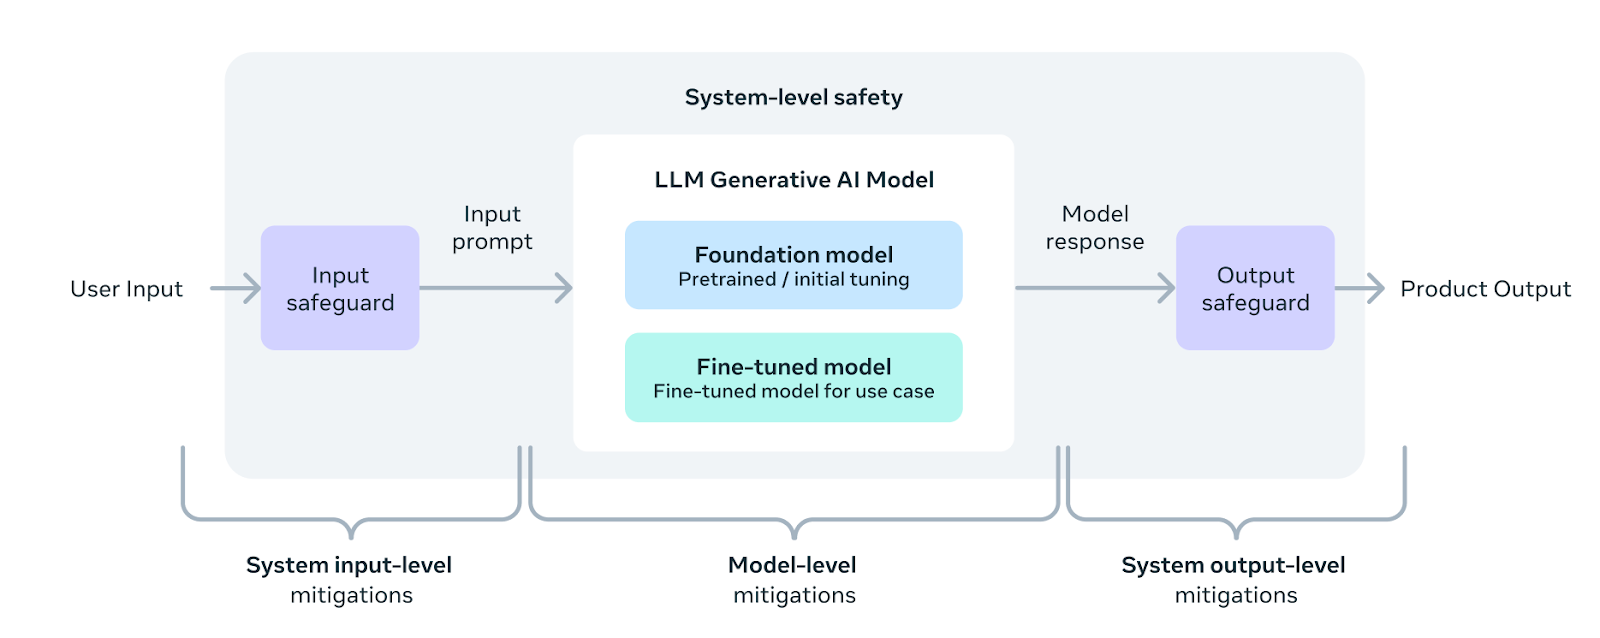
\includegraphics[width=\linewidth]{img/LLAMA/llama.png}
    \caption*{Fonte: Meta AI \cite{llama3blog}}
    \label{fig:llama1}
\end{figure}

O \textit{fine tuning} é necessário ser realizado para o caso especifico de uso, além do \textit{fine tuning} da propria geração do modelo após o pré-treino. Assim como o BERT, o LLama se torna flexível para adaptações e contextos diversos da área de \textit{Natural Language Processing} (NLP).

\subsubsection{Limitações}
Um dos principais fatores de desvantagens do LLama reportado por usuários, é a possibilidade do modelo gerar respostas imprecisas ou alucinações em cenários de alta mutabilidade, o que torna o modelo diante de uma maior necessidade de receber um contexto prévio para a geração de uma resposta assertiva. Por isso que num \textit{pipeline} de RAG, a ideia é que esse conteúdo contextual seja inserido no momento da reposta da inferência do modelo, reduzindo assim as alucinações.

